\section{Conclusion}

In this paper the Hashed Shading algorithm has been presented and evaluated. Hashed Shading is
a light assignment algorithm which subdivides the scene space independently of the
view frustum. This subdivision is then stored in a linkless octree which can be queried during
shading. Because the subdivision is independent of the view frustum, changes in the camera
position and orientation do not require a complete recalculation of the data structures. Thus the
data structures can be reused between frames.

The Hashed Shading algorithm performs better than the Tiled Shading algorithm and
approaches the reduction of light calculations achieved by Clustered Shading.
Furthermore Hashed Shading performs slightly better with increasing resolutions
compared to both Tiled and Clustered Shading, because its subdivision does not
depend directly on the direction.

However there are still two major problems with the current Hashed Shading implementation.
The memory footprint increases cubicly with a decreasing node size. This leads
to unacceptable memory requirements for small node sizes. Secondly, dynamic lights
are not currently not supported within the Hashed Shading implementation. Adding
this support would increase computation time during shading.

Overall, it can be concluded that camera-independent light assignment is a viable strategy.
The decoupling of resolution could play a role with the trend of increasing screen resolutions.
Future work would need to solve the memory requirements and allow for efficient support
of dynamic lights in order for Hashed Shading and similar algorithms to be competitive with
Clustered Shading.

% In this paper we have presented and evaluated the Hashed Shading algorithm. In Hashed Shading
% the scene space is divided independent of the camera with a linkless octree data structure.
% The linkless octree allows for efficient light assignment and reuse of data structures between
% frames. We have shown that it is possible to achieve better performance than Tiled Shading
% by using this camera-independent data structure. Furthermore for small node sizes, the
% number of light calculations approaches that of Clustered Shading, and could potentially
% exceed it. There are two problems with the current implementation of Hashed Shading;
% no dynamic lights are supported and the memory footprint is large. These two issues need
% to be addressed before Hashed Shading becomes a viable alternative for Tiled and Clustered
% Shading.

\section{Future work}

The two main issues with the current implementation of Hashed Shading are the large memory
footprint and the lack of support for dynamic lights. These two issues have to be addressed
before Hashed Shading can become a viable alternative to Clustered Shading. Proposals
to solve those two issues are introduced in the next sections.

Besides these two issues, there are several other directions for future work. Currently
the Hashed Shading implementation only supports point lights. In order to support
other light types, strategies to convert their light volumes into octrees need to be
drafted. The current implementation also does not support shadows currently. There
are several algorithms which leverage the clustered shading clusters to reduce
the amount of work required to support shadows within Clustered Shading\cite{Olsson:2014:EVS:2556700.2556701, kampe2016fast}.
Similar approaches could be used to support shadows in Hashed Shading by leveraging
the octree data structure.

% Besides these two issues there are several other options for future work. Currently
% the Hashed Shading algorithm only supports point lights, in order to support other
% lights, their volumes need to be represented as octrees efficiently. Secondly
% the current implementation has no support for shadows. There are several ways in which
% the Clustered Shading clusters are leveraged to reduce the work required to calculate
% shadows\cite{}. Similar techniques could be developed by using the Hashed Shading octree.

\subsection{Memory Usage Reduction}
\subsubsection{Geometry}

\begin{figure}[t]
  \centering
  \begin{subfigure}[b]{0.249\textwidth}
    \centering
  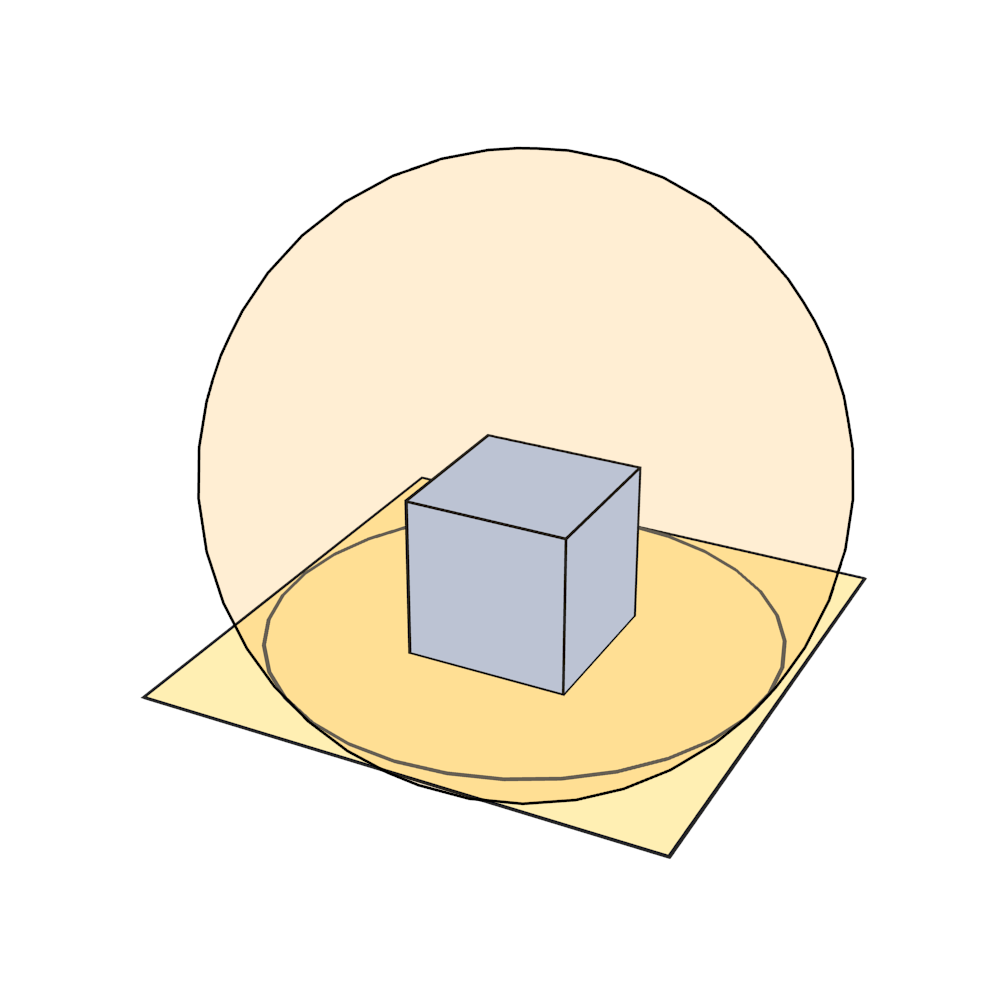
\includegraphics[width=\textwidth]{./img/raw/besluit-geom/scene.png}
  \caption{Simple scene.}
  \label{fig:vo-geometrie:0}
  \end{subfigure}%
  \begin{subfigure}[b]{0.249\textwidth}
    \centering
  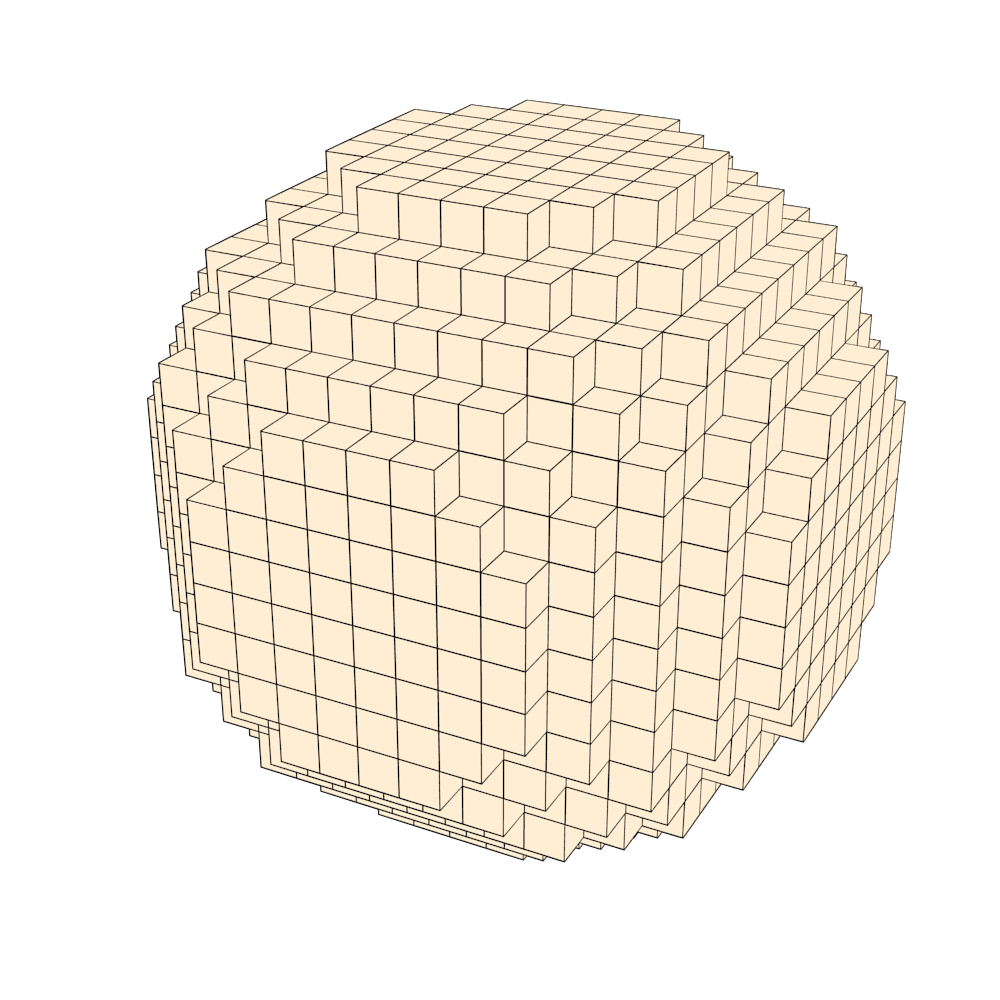
\includegraphics[width=\textwidth]{./img/raw/besluit-geom/light.png}
  \caption{Light nodes.}
  \label{fig:vo-subsets:1}
  \end{subfigure}\\
  \begin{subfigure}[b]{0.249\textwidth}
    \centering
  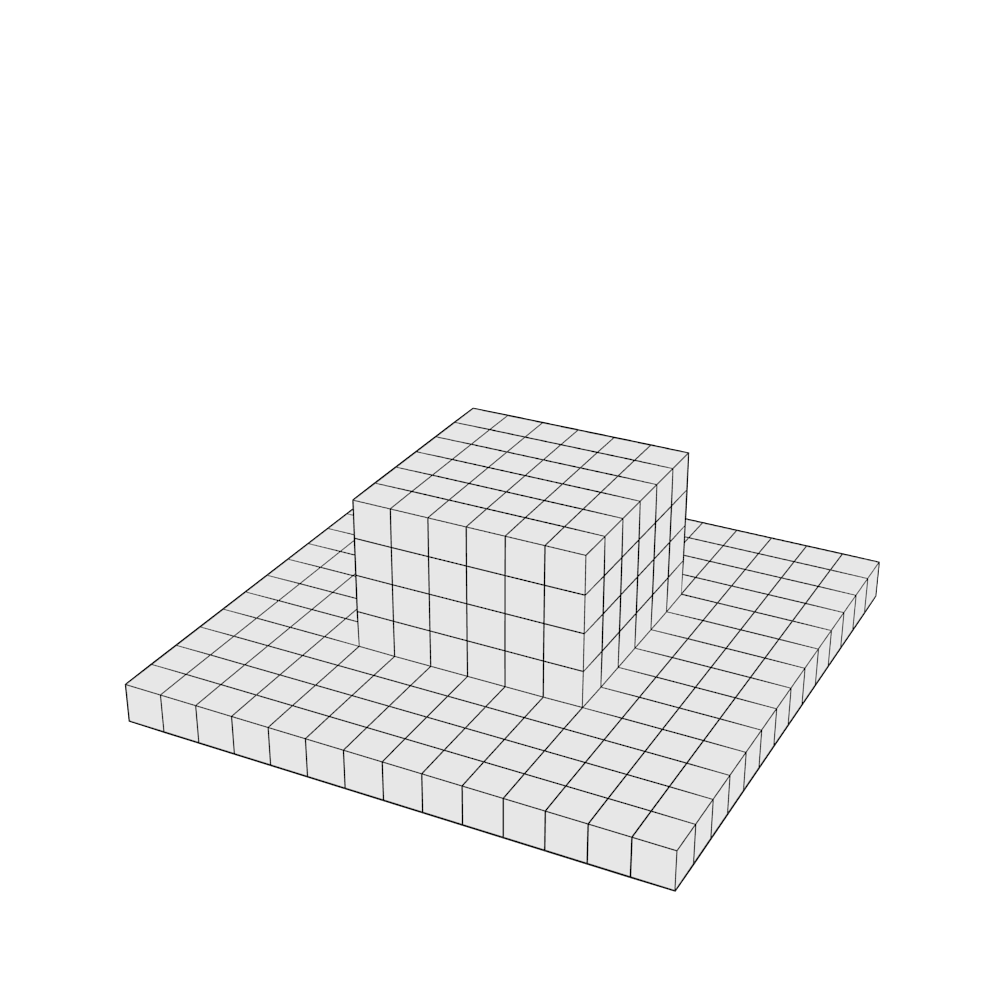
\includegraphics[width=\textwidth]{./img/raw/besluit-geom/geom.png}
  \caption{Geometry nodes.}
  \label{fig:vo-geometrie:0}
  \end{subfigure}%
  \begin{subfigure}[b]{0.249\textwidth}
    \centering
  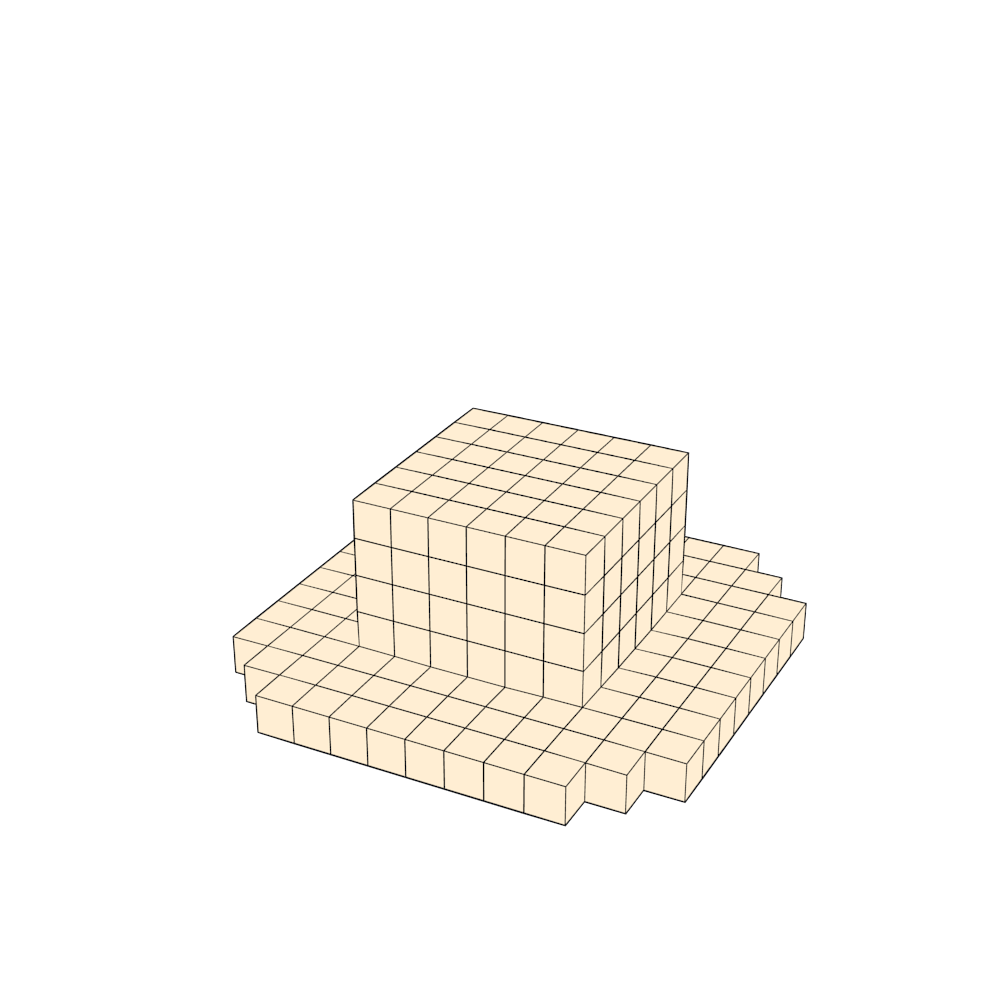
\includegraphics[width=\textwidth]{./img/raw/besluit-geom/comb.png}
  \caption{Light geometry nodes.}
  \label{fig:vo-subsets:1}
  \end{subfigure}
  \caption{Reduction of the number of nodes by excluding empty space.}
  \label{fig:vo-geometrie}
\end{figure}


An important insight Clustered Shading uses to reduce memory usage is that only clusters
which contain geometry will potentially be queried. Thus only clusters that contain potential
samples need to be constructed and kept in memory. This reduces the total number of clusters
required by Clustered Shading. This insight can also be leveraged by Hashed Shading. There
is no need to keep nodes which contain no geometry in memory as they will never be queried.
If a second octree with the same origin and size of the screen octree is constructed, where
the leaf nodes specify whether the corresponding volumes contains geometry, then this octree
can be used to filter out nodes which will not be queried. Only if a node contains both
geometry and light information, it needs to be stored in the linkless octree. Thus such
a geometry octree could be used to greatly reduce the number of nodes in the linkless octree as
is shown in figure \ref{fig:vo-geometrie}.

A second advantage of such an approach would be that the number of nodes would not necessarily
be cubicly dependent on the node size. A smaller node size would also increase the precision
with which geometry is represented, thus it would reduce the space which contains geometry and
therefore reduce the increase in number of nodes which need to be represented within the linkless
octree.

% An important insight Clustered Shading leverages to reduce the memory usage is that samples
% will only be generated in clusters that contain geometry. Thus there is no need to construct
% clusters that will not generate samples. A similar approach can be used in Hashed Shading.
% A second octree with the same size and origin can be constructed for the geometry, where in
% the leaf node is stored if the corresponding volume contains geometry. This octree can then
% be used to determine whether a node has to be saved or not. Only if a node contains geometry
% it needs to be physically saved, and only if the node contains both lights and geometry it
% needs to be saved in the second spatial hash function. Thus such an octree could greatly
% reduce the number of nodes as is shown in figure \ref{fig:vo-geometrie}.

% A second advantage of this approach would be that a smaller node size would not directly
% cubicly increase the number of nodes. As a smaller node size would also increase the
% precision with which the geometry is represented, it would actually increase the amount of
% empty space, thus reducing the amount of nodes that need to be kept in memory.

Lastly the conditions required for a set of sibling nodes to be combined into a single
leaf node in the preceding layer could be weakened. Since nodes which do not contain any
geometry data will never be queried, an arbitrary value could be assigned to them, without
influencing the performance of Hashed Shading. The current condition requires all the sibling
nodes to have the same set of lights, before they can be combined into a single leaf node. With
this optimisation this can be weakened to requiring to all sibling nodes which contain geometry
to contain an equal set of lights. This would further reduce the number of nodes
needed to represent the scene space.

\subsubsection{Subdivision of Space}

\begin{figure}
  \usetikzlibrary{shapes.arrows, positioning}
  \definecolor{LightColor}{rgb}{1.0,0.901,0.805}
  \definecolor{EmptyColor}{HTML}{DCE2E6}

  \definecolor{tile0}{HTML}{DABDE4}
  \definecolor{tile1}{HTML}{B8DBF4}
  \definecolor{tile2}{HTML}{B5EDCD}
  \definecolor{tile3}{HTML}{FBEBA7}
  \definecolor{tile4}{HTML}{F9C1BB}
  \definecolor{tile5}{rgb}{1, 1, 1}

  \tikzstyle{array_element}=[rectangle,
                             minimum height=0.5cm, 
                             minimum width=0.5cm, 
                             minimum size=0.5cm,
                             draw=black,
                             rounded corners=2.5, ]
  \tikzstyle{empty_element}=[rectangle,
  fill=white
                                ]


  \begin{adjustbox}{minipage=\textwidth, scale=0.425}
    \centering
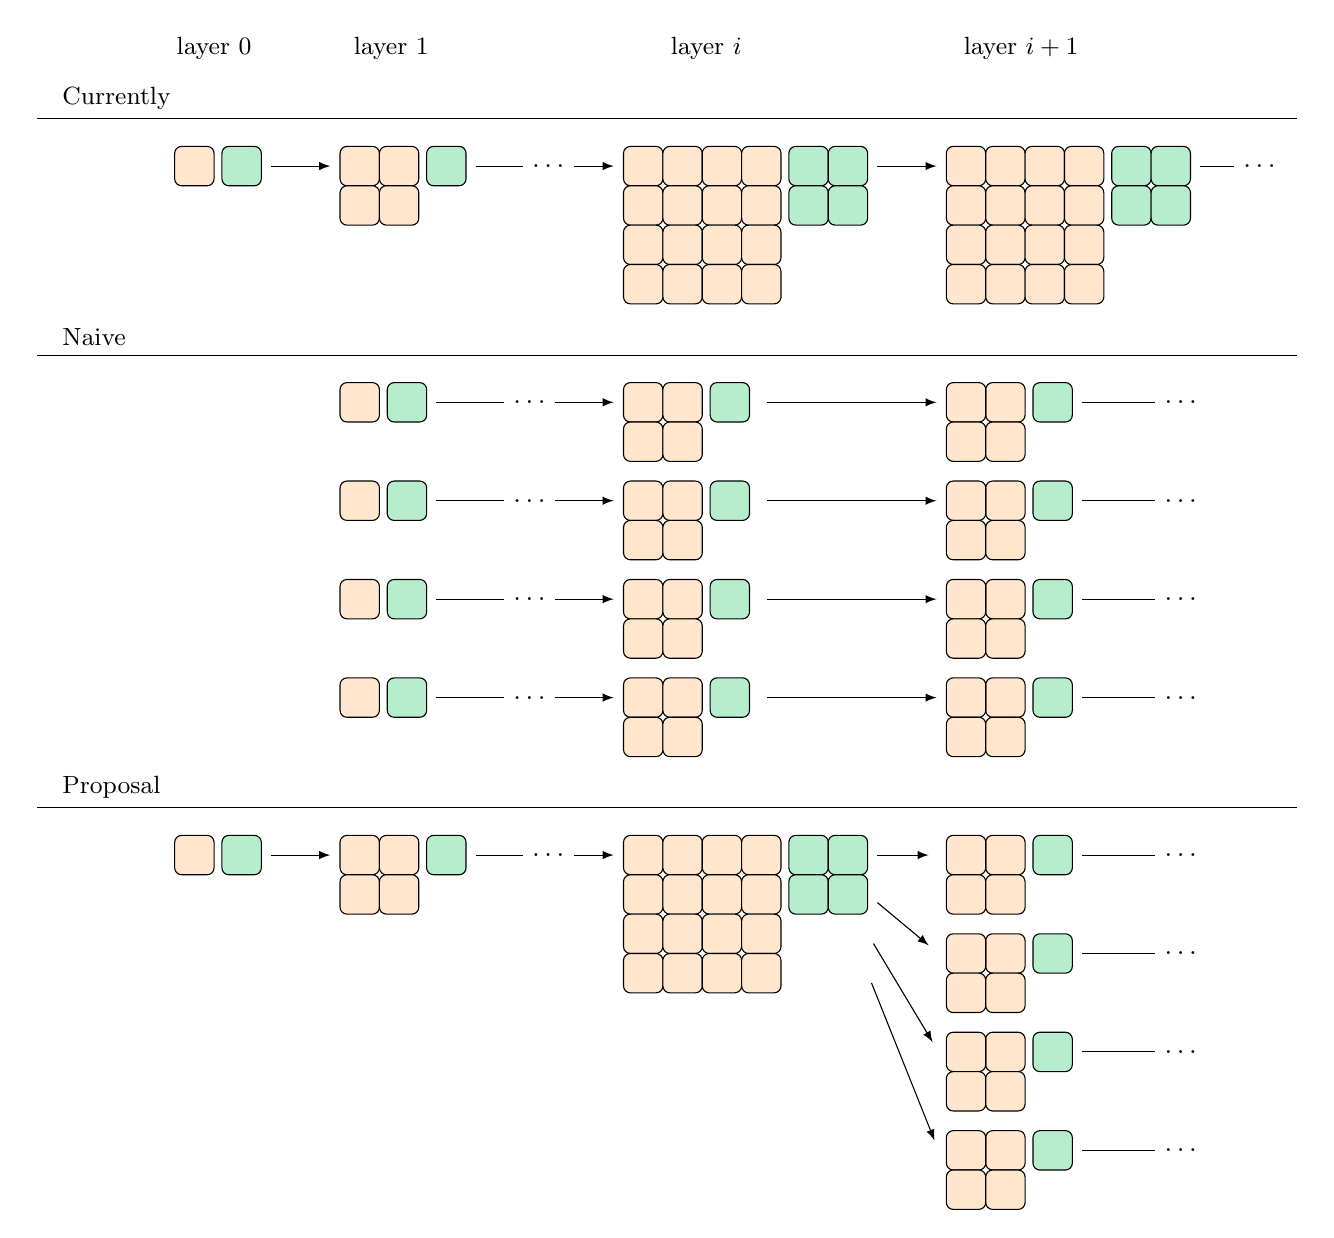
\begin{tikzpicture}
     \node at (0.5cm * 0 + 0.1cm * 0, 0) (H) [array_element, fill=LightColor] {};
     \node at (0.5cm * 1 + 0.1cm * 1, 0) (H) [array_element, fill=tile2] {};

     \node at (0.5cm * 1 + 0.1cm * 1 + 1.5cm * 1, 0) (H) [array_element, fill=LightColor] {};
     \node at (0.5cm * 2 + 0.1cm * 1 + 1.5cm * 1, 0) (H) [array_element, fill=LightColor] {};
     \node at (0.5cm * 1 + 0.1cm * 1 + 1.5cm * 1, -0.5cm) (H) [array_element, fill=LightColor] {};
     \node at (0.5cm * 2 + 0.1cm * 1 + 1.5cm * 1, -0.5cm) (H) [array_element, fill=LightColor] {};
     
     \node at (0.5cm * 3 + 0.1cm * 2 + 1.5cm * 1, -0.0cm) (H) [array_element, fill=tile2] {};

    \node at (0.5cm * 1 + 0.1cm * 1 + 0.25cm, -0.cm) (c1) [] {};
    \node at (0.5cm * 1 + 0.1cm * 1 + 1.5cm * 1 - 0.25cm, -0.cm) (c2) [] {};
    \draw[-latex](c1) -- (c2);

    \node at (0.5cm * 3 + 0.1cm * 2 + 1.5cm * 1 + 0.25cm, -0.cm) (c1) [] {};
    \node at (0.5cm * 3 + 0.1cm * 2 + 1.5cm * 1 + 2.5cm - 0.25cm, -0.cm) (c2) [] {};
    \draw[-latex](c1) --node[empty_element, pos=0.525] {$\dots$} (c2);

    \node at (0.5cm * 8 + 0.1cm * 3 + 1.5cm * 1 + 2.5cm + 0.25cm, -0.cm) (c1) [] {};
    \node at (0.5cm * 8 + 0.1cm * 3 + 1.5cm * 2 + 2.5cm - 0.25cm, -0.cm) (c2) [] {};
    \draw[-latex](c1) -- (c2);

    \node at (0.5cm * 16 + 0.1cm * 4 + 1.5cm * 1 + 2.5cm + 0.25cm, -0.cm) (c1) [] {};
    \node at (0.5cm * 16 + 0.1cm * 4 + 1.5cm * 2 + 2.5cm - 0.25cm, -0.cm) (c2) [] {};
    \draw[-](c1) --node[empty_element, pos=1] {$\dots$} (c2);



    \foreach \la in {0,...,3} {
        \foreach \lb in {0,...,3} {
            \node at (0.5cm * \la + 0.5cm * 3 + 0.1cm * 2 + 1.5cm * 1 + 2.5cm, -0.5cm * \lb) (H\la\lb) [array_element, fill=LightColor] {};
        }
    }
    \foreach \la in {0,...,1} {
        \foreach \lb in {0,...,1} {
            \node at (0.5cm * \la + 0.5cm * 7 + 0.1cm * 3 + 1.5cm * 1 + 2.5cm , -0.5cm * \lb) (H\la\lb) [array_element, fill=tile2] {};
        }
    }

    \foreach \la in {0,...,3} {
        \foreach \lb in {0,...,3} {
            \node at (0.5cm * \la + 0.5cm * 8 + 0.1cm * 3 + 1.5cm * 2 + 2.5cm, -0.5cm * \lb) (H\la\lb) [array_element, fill=LightColor] {};
        }
    }
    \foreach \la in {0,...,1} {
        \foreach \lb in {0,...,1} {
            \node at (0.5cm * \la + 0.5cm * 12 + 0.1cm * 4 + 1.5cm * 2 + 2.5cm , -0.5cm * \lb) (H\la\lb) [array_element, fill=tile2] {};
        }
    }



      \foreach \la in {0,...,3} {
        \node at (0.5cm * 2 + 0.1cm * 1 + 1.0cm, -3cm - 1.25cm * \la) (H) [array_element, fill=LightColor] {};
        \node at (0.5cm * 3 + 0.1cm * 2 + 1.0cm, -3cm - 1.25cm * \la) (H) [array_element, fill=tile2] {};
        
             \node at (0.5cm * 0 + 0.1cm * 2 + 1.5cm * 2 + 2.5cm, -3cm -1.25cm * \la) (H) [array_element, fill=LightColor] {};
     \node at (0.5cm * 1 + 0.1cm * 2 + 1.5cm * 2  + 2.5cm, -3cm -1.25cm * \la) (H) [array_element, fill=LightColor] {};
     \node at (0.5cm * 0 + 0.1cm * 2 + 1.5cm * 2 + 2.5cm, -0.5cm -3cm -1.25cm * \la) (H) [array_element, fill=LightColor] {};
     \node at (0.5cm * 1 + 0.1cm * 2 + 1.5cm * 2 + 2.5cm, -0.5cm - 3cm -1.25cm * \la) (H) [array_element, fill=LightColor] {};
     \node at (0.5cm * 2 + 0.1cm * 3 + 1.5cm * 2 + 2.5cm, -0.0cm - 3cm -1.25cm * \la) (H) [array_element, fill=tile2] {};
     
         \node at (0.5cm * 2 + 0.1cm * 2 + 1.5cm * 1 + 0.25cm, -0.cm - 3cm -1.25cm * \la) (c1) [] {};
    \node at (0.5cm * 3 + 0.1cm * 2 + 1.5cm * 1 + 2.5cm - 0.25cm, -0.0cm - 3cm -1.25cm * \la) (c2) [] {};
    \draw[-latex](c1) --node[empty_element, pos=0.525] {$\dots$} (c2);

     \node at (0.5cm * 6 + 0.1cm * 3 + 1.5cm * 3 + 2.5cm, -3cm -1.25cm * \la) (H) [array_element, fill=LightColor] {};
     \node at (0.5cm * 5 + 0.1cm * 3 + 1.5cm * 3  + 2.5cm, -3cm -1.25cm * \la) (H) [array_element, fill=LightColor] {};
     \node at (0.5cm * 5 + 0.1cm * 3 + 1.5cm * 3 + 2.5cm, -0.5cm -3cm -1.25cm * \la) (H) [array_element, fill=LightColor] {};
     \node at (0.5cm * 6 + 0.1cm * 3 + 1.5cm * 3 + 2.5cm, -0.5cm - 3cm -1.25cm * \la) (H) [array_element, fill=LightColor] {};
     \node at (0.5cm * 7 + 0.1cm * 4 + 1.5cm * 3 + 2.5cm, -0.0cm - 3cm -1.25cm * \la) (H) [array_element, fill=tile2] {};

    \node at (0.5cm * 2 + 0.1cm * 4 + 1.5cm * 2 + 2.5cm + 0.25cm, -0.cm -3cm -1.25cm * \la) (c1) [] {};
    \node at (0.5cm * 5 + 0.1cm * 3 + 1.5cm * 3 + 2.5cm - 0.25cm, -0.cm-3cm -1.25cm * \la) (c2) [] {};
    \draw[-latex](c1) -- (c2);

    \node at (0.5cm * 16 + 0.1cm * 4 + 1.5cm * 1 + 2.5cm + 0.25cm - 1.5cm, -3cm -1.25cm * \la) (c1) [] {};
    \node at (0.5cm * 16 + 0.1cm * 4 + 1.5cm * 2 + 2.5cm - 0.25cm - 1cm, -3cm -1.25cm * \la) (c2) [] {};
    \draw[-](c1) --node[empty_element, pos=1] {$\dots$} (c2);
      }

     \node at (0.5cm * 0 + 0.1cm * 0, 0 - 8.75cm) (H) [array_element, fill=LightColor] {};
     \node at (0.5cm * 1 + 0.1cm * 1, 0- 8.75cm) (H) [array_element, fill=tile2] {};

     \node at (0.5cm * 1 + 0.1cm * 1 + 1.5cm * 1, 0- 8.75cm) (H) [array_element, fill=LightColor] {};
     \node at (0.5cm * 2 + 0.1cm * 1 + 1.5cm * 1, 0 - 8.75cm) (H) [array_element, fill=LightColor] {};
     \node at (0.5cm * 1 + 0.1cm * 1 + 1.5cm * 1, -0.5cm - 8.75cm) (H) [array_element, fill=LightColor] {};
     \node at (0.5cm * 2 + 0.1cm * 1 + 1.5cm * 1, -0.5cm - 8.75cm) (H) [array_element, fill=LightColor] {};
     
     \node at (0.5cm * 3 + 0.1cm * 2 + 1.5cm * 1, -0.0cm - 8.75cm) (H) [array_element, fill=tile2] {};

    \node at (0.5cm * 1 + 0.1cm * 1 + 0.25cm, -0.cm - 8.75cm) (c1) [] {};
    \node at (0.5cm * 1 + 0.1cm * 1 + 1.5cm * 1 - 0.25cm, -0.cm - 8.75cm) (c2) [] {};
    \draw[-latex](c1) -- (c2);

    \node at (0.5cm * 3 + 0.1cm * 2 + 1.5cm * 1 + 0.25cm, -0.cm - 8.75cm) (c1) [] {};
    \node at (0.5cm * 3 + 0.1cm * 2 + 1.5cm * 1 + 2.5cm - 0.25cm, -0.cm - 8.75cm) (c2) [] {};
    \draw[-latex](c1) --node[empty_element, pos=0.525] {$\dots$} (c2);

    \node at (0.5cm * 8 + 0.1cm * 3 + 1.5cm * 1 + 2.5cm + 0.25cm, -0.cm - 8.75cm) (c1) [] {};
    \node at (0.5cm * 8 + 0.1cm * 3 + 1.5cm * 2 + 2.5cm - 0.35cm, -0.cm - 8.75cm) (c2) [] {};
    \draw[-latex](c1) -- (c2);
    
        \node at (0.5cm * 8 + 0.1cm * 3 + 1.5cm * 1 + 2.5cm + 0.25cm, -0.cm - 8.75cm - 0.5cm) (c1) [] {};
    \node at (0.5cm * 8 + 0.1cm * 3 + 1.5cm * 2 + 2.5cm - 0.35cm, -0.cm - 8.75cm - 1.25 cm) (c2) [] {};
    \draw[-latex](c1) -- (c2);

        \node at (0.5cm * 8 + 0.1cm * 3 + 1.5cm * 1 + 2.5cm + 0.25cm, -0.cm - 8.75cm  - 0.5cm * 2) (c1) [] {};
    \node at (0.5cm * 8 + 0.1cm * 3 + 1.5cm * 2 + 2.5cm - 0.35cm, -0.cm - 8.75cm - 1.25 cm * 2) (c2) [] {};
    \draw[-latex](c1) -- (c2);

        \node at (0.5cm * 8 + 0.1cm * 3 + 1.5cm * 1 + 2.5cm + 0.25cm, -0.cm - 8.75cm - 0.5cm * 3) (c1) [] {};
    \node at (0.5cm * 8 + 0.1cm * 3 + 1.5cm * 2 + 2.5cm - 0.35cm, -0.cm - 8.75cm - 1.25 cm * 3) (c2) [] {};
    \draw[-latex](c1) -- (c2);


        \foreach \la in {0,...,3} {
        \foreach \lb in {0,...,3} {
            \node at (0.5cm * \la + 0.5cm * 3 + 0.1cm * 2 + 1.5cm * 1 + 2.5cm, -0.5cm * \lb - 8.75cm) (H\la\lb) [array_element, fill=LightColor] {};
        }
    }
    \foreach \la in {0,...,1} {
        \foreach \lb in {0,...,1} {
            \node at (0.5cm * \la + 0.5cm * 7 + 0.1cm * 3 + 1.5cm * 1 + 2.5cm , -0.5cm * \lb - 8.75cm) (H\la\lb) [array_element, fill=tile2] {};
        }
    }
    \foreach \la in {0,...,3} {
         \node at (0.5cm * 6 + 0.1cm * 3 + 1.5cm * 3 + 2.5cm, -3cm -1.25cm * \la - 5.75cm) (H) [array_element, fill=LightColor] {};
     \node at (0.5cm * 5 + 0.1cm * 3 + 1.5cm * 3  + 2.5cm, -3cm -1.25cm * \la - 5.75cm) (H) [array_element, fill=LightColor] {};
     \node at (0.5cm * 5 + 0.1cm * 3 + 1.5cm * 3 + 2.5cm, -0.5cm -3cm -1.25cm * \la - 5.75cm) (H) [array_element, fill=LightColor] {};
     \node at (0.5cm * 6 + 0.1cm * 3 + 1.5cm * 3 + 2.5cm, -0.5cm - 3cm -1.25cm * \la - 5.75cm) (H) [array_element, fill=LightColor] {};
     \node at (0.5cm * 7 + 0.1cm * 4 + 1.5cm * 3 + 2.5cm, -0.0cm - 3cm -1.25cm * \la - 5.75cm) (H) [array_element, fill=tile2] {};
    \node at (0.5cm * 16 + 0.1cm * 4 + 1.5cm * 1 + 2.5cm + 0.25cm - 1.5cm, -3cm -1.25cm * \la - 5.75cm) (c1) [] {};
    \node at (0.5cm * 16 + 0.1cm * 4 + 1.5cm * 2 + 2.5cm - 0.25cm - 1cm, -3cm -1.25cm * \la - 5.75cm) (c2) [] {};
    \draw[-](c1) --node[empty_element, pos=1] {$\dots$} (c2);




    }
    \node at (-2.0cm, 0.6cm) (line-1-l) {};
    \node at (14cm, 0.6cm) (line-1-r) {};
    \draw[-, thin] (line-1-l.center) -- (line-1-r.center) node[pos=0.0125, above right] {\small Currently};
    
    \node at (-2.0cm, 0.6cm - 3cm) (line-1-l) {};
    \node at (14cm, 0.6cm - 3cm) (line-1-r) {};
    \draw[-, thin] (line-1-l.center) -- (line-1-r.center) node[pos=0.0125, above right] {\small Naive};
    
\node at (-2.0cm, 0.6cm - 5cm - 3 * 1.25cm) (line-1-l) {};
\node at (14cm, 0.6cm - 5cm - 3 * 1.25cm) (line-1-r) {};
    \draw[-, thin] (line-1-l.center) -- (line-1-r.center) node[pos=0.0125, above right] {\small Proposal};

\node at (0.25cm, 1.5cm) (laag0) {\small layer $0$};
\node at (0.25cm + 2.25cm, 1.5cm) (laag0) {\small layer $1$};
\node at (0.25cm + 6.25cm, 1.5cm) (laag0) {\small layer $i$};
\node at (0.25cm + 10.25cm, 1.5cm) (laag0) {\small layer $i + 1$};

\end{tikzpicture}
\end{adjustbox}
  \caption{Subdivision strategy deeper layers of the linkless octree.}
  \label{fig:vo-textures}
\end{figure}


A common approach in many graphical applications is to only load data into memory which
is visible, i.e. only that which falls within the view frustum. In the current implementation
the whole scene is loaded into memory, without any regard for the view frustum, which leads
to an unnecessary large memory usage. If the view frustum is significantly smaller than the
whole scene, it can be advantageous to subdivide the light assignment octree in chunks, and
only load the visible chunks into memory. If the chunk size is set to be similar to the view
frustum, at least eight chunks are required to cover the view frustum at any point.
This could be extended to 27 chunks if camera rotations are common. In this case no new chunks
will have to be loaded in when the camera orientation changes, thus reducing the texture
bandwidth. When these chunks require less memory than the complete representation, the memory
usage is reduced.

A potential problem of this approach is the large number of textures required to represent
the octree. Each layer of each chunk would require two separate textures, four if the layer
also contains leaf nodes. If 27 chunks are used, and each chunk uses several layers, this
would quickly lead to an infeasible amount of textures. However looking at the results of
the memory usage, it can be shown that the majority of the memory is used in the deeper
layers, which contain a large number of nodes, and that the shallow layers are relatively
small. An alternative would be to only subdivide the space into chunks at a certain depth.
In the current implementation each layer represents the full scene space, however there is
no obstacle into subdividing this space into smaller chunks. If we would subdivide layer $l + 1$
into chunks, then the branch nodes in layer $l$ would only require a single value to identify
the chunk in which the child node lays. This would make it possible to reduce the memory usage
in the deeper layers, while keeping the number of changing textures to a minimum.
The possible options are shown in figure \ref{fig:vo-textures}.

Finally, the chunk approach would make it trivial to support level of detail. Objects close
to the camera will generally take up more screen space than objects further away from the camera,
due to perspective. Thus if the same reduction of light calculations is created for objects
far away from the camera as for objects close by the camera, the amount of memory used to reduce
the number of lights for samples far away will be relatively greater. By reducing the amount of
memory used for space further away from the camera, and increasing it for space close to the
camera, a greater reduction of light calculations overall can be achieved. In Clustered
Shading this is done by scaling the cluster volume with regards to the camera's $z$-axis.

The linkless octree could support this level of detail by defining multiple spatial hash functions
per layer. When a chunk is loaded close to the camera, the regular spatial hash functions would
be loaded. For chunks further from the camera, only layers till a certain value could be loaded
in, where the last loaded layer contains only leaf nodes. Thus per layer one regular spatial hash function
and one spatial hash function only containing leaf nodes would have to be defined.

\subsection{Dynamic Light Support}

The second issue of the current implementation of Hashed Shading is the lack of support for
dynamic lights. The downside of not rebuilding data structures per frame is that changes
in lights are not implicitly reflected in the data structures any more. Supporting dynamic
lights would thus always increase the amount of work per frame.
Games and other real-time applications generally have a high frame rate, between 30 and 60 frames
per second, therefore changes in lights are generally small and local. This could be leveraged
to efficiently update the Hashed Shading data structures.
The bottleneck operation in the construction of the Hashed Shading data structures is the construction of the
spatial hash functions of the layers of the octree. In order to efficiently support dynamic lights,
these operations thus need to be kept to a minimum. A spatial hash function needs to be rebuild if
a new node is added that collides with an existing value:

\begin{equation*}
    H\left[ \mathit{h}_0\left(\mathbf{k}\right) + \Phi\left[ \mathit{h}_1\left(\mathbf{k}\right) \right] \right] \neq \varnothing 
\end{equation*}

\noindent where $\mathbf{k}$ is the position of a new node. In all other cases the existing
textures can be updated without a complete recalculation of the spatial hash function of a layer.

There are two situations which require the addition of nodes in layers. If a light index is added
to a previously empty node, a new data element needs to be added to the data hash function of a layer.
When a leaf node gets subdivided into eight child nodes, a new node is added to the first
spatial hash function of the next layer describing these eight child nodes, and for each of the child
nodes that contain data, the data nodes are added to the data spatial hash function of the next layer.
The subdivision of nodes therefore is the most likely source of recalculations.

It might prove efficient to slightly extend the size of the hash tables to increase the amount
of empty space within them. While this would increase the memory foot print, it could greatly reduce the
number of times a spatial hash function needs to be recalculated. The effects of such a change
would be interesting to explore.

In the current implementation the whole space of each layer is globally linked, therefore a local
change of a single light might require the complete space to be recalculated. Currently the implementation
can not take advantage of the local nature of light changes. If the support of dynamic lights is combined
with the chunk optimisation, only the chunks affected by a light change need to be updated, reducing the
space affected by that change. Furthermore, because the construction
time of a spatial hash functions is directly linked to its size, recalculating the spatial hash function
of a chunk would be smaller than recalculating the spatial hash function of the complete space, 
further reducing the amount of time needed to update.
Lastly, only chunks that are currently in memory need to be updated immediately, as changes to these
chunks are directly visible. Changes to chunks that are not currently loaded on the GPU will not be visible
until the chunk is loaded in GPU memory. Changes to invisible chunks can be queued, and only executed
once the chunk has to be loaded into memory. This would reduce the bandwidth and potentially the
execution time.

